\ifbook{
  \mysubsubsection{Le Web}
  \paragraph{} Avec l'arrivée des technologies du "Web", soit essentiellement au début HTML et HTTP,
  le mouvement de balancier évoqué dans une précédente section s'inverse de nouveau. Dans leurs
  laboratoires, les concepteurs initiaux de ce protocole de communication visèrent avant tout la
  simplicité pour assurer surtout une bonne compatibilité entre les différents systèmes existants
  de part le monde.

  \paragraph{} En effet, avant d'aller plus loin, il est important de se rappeler que à cette
  époque, il existait de nombreux systèmes d'exploitation, tous différents et rarement interopérables
  entre eux. Les plus connus aujourd'hui sont Apple et Windows, mais à l'époque s'ajoutaient aussi de
  nombreux types d'Unix différents (cf. \textit{\mylink{http://en.wikipedia.org/wiki/Unix\_wars}{Unix
  Wars}}), accompagnés par de nombreux autres systèmes, tel que OpenVMS.

  \paragraph{} Sans compter que ces systèmes avaient même des protocoles de communications
  différents. Pour reprendre l'exemple de OpenVMS, ce système utilisait un protocole propriétaire à
  son constructeur, intitulé DecNet et non le standard \textit{de facto} d'aujourd'hui, le protocole
  TCP/IP.

  \paragraph{} Ainsi, concevoir un système applicatif portable - c'est à dire qui fonctionnerait à
  peu près partout et permettrait de communiquer aisément entre des systèmes différents n'était pas
  une simple tâche. C'est donc en partie pour ces raisons, que les concepteurs de HTTP et de HTML
  ont choisi de faire très simple.

  \paragraph{} Le protocole en lui-même est un simple protocole \textbf{texte}, et non binaire, il
  est donc aisé de l'implémenter et, au besoin, de regarder l'échange en lui même pour comprendre la
  source d'un problème. Comme les données échangées sont du texte, tout système de l'époque, aussi
  différent soit-il des autres, était capable de le comprendre.
}

\ifslide{
  \demoframe{Le protocole HTTP}{
    \begin{block}{Démonstrations}
      \begin{itemize}
        \item simple connection avec telnet
        \item connection complète avec les \textit{Developers tools} de Google Chrome
      \end{itemize}
    \end{block}

    \begin{center}
      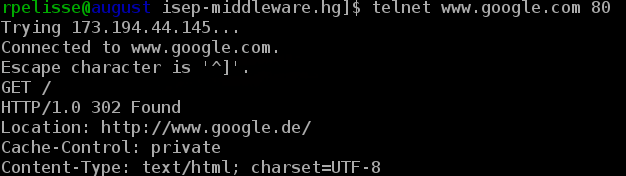
\includegraphics[scale=0.5]{img/telnet-google.png}
    \end{center}
  }
}

\ifbook{

  \paragraph{} Toujours par souci de simplicité, l'objectif était dans les faits assez peu ambitieux,
  puisqu'il s'agissait d'afficher du contenu simple, du texte un peu enrichi, pour permettre en fait
  au milieu universitaire de publier, facilement et rapidement,  à l'intention de leurs confrères,
  des informations.

  \paragraph{} La conséquence directe de ce choix simple de données utilisées à été de limiter le
  rôle du client à afficher, du mieux possible selon le système utilisée, les informations
  fournies par le serveur HTTP. Le \textbf{client lourd} venait de faire un régime et redevenait un
  \textbf{client léger}.

  \begin{figure}[h]
    \begin{center}
      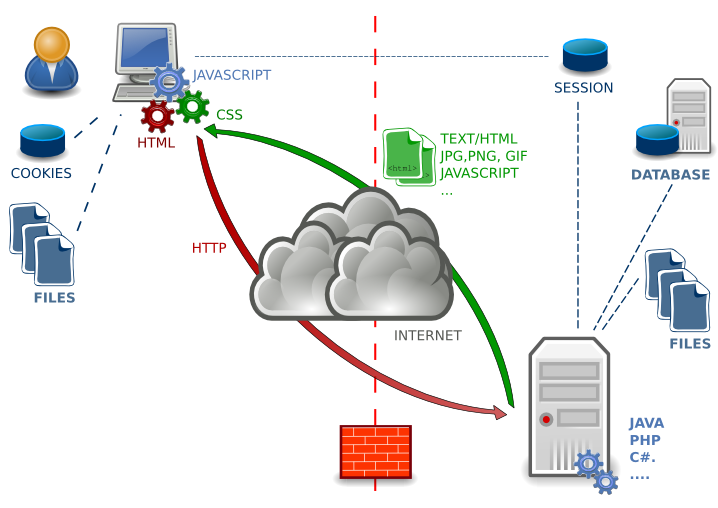
\includegraphics[scale=0.3]{img/internet.png}
      \caption{Extrait de code HTML contenant du Javascript et du CSS}
      \label{internet}
    \end{center}
  \end{figure}
}

\ifslide {
  \begin{frame}{Le "Web"}
    \begin{center}
      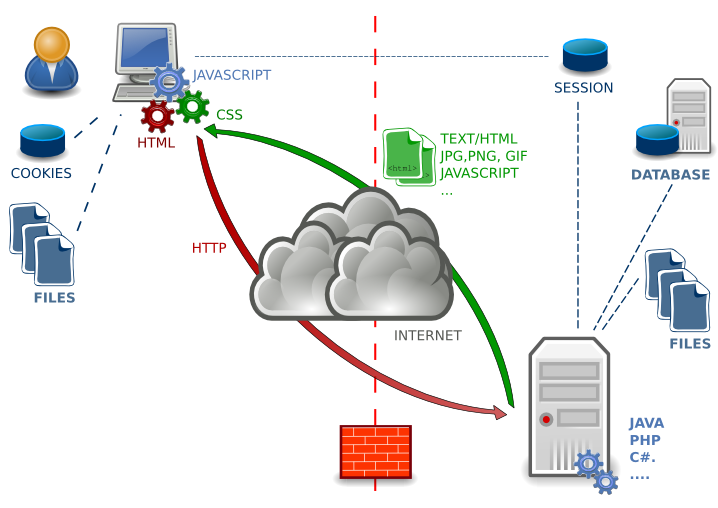
\includegraphics[scale=0.3]{img/internet.png}
    \end{center}
  \end{frame}
}

\ifbook{
  \mysubsubsection{Les technologies "Web" s'enrichissent}
  \mysubsubsubsection{Formulaire et session HTTP}

  \paragraph{} Le protocole HTTP, et son format de données, HTML, a eu le succès qu'on connaît, et
  rapidement, malgré l'élégance de la simplicité de la solution, il apparut clair que l'\textbf{absence
  d'interaction} entre l'utilisateur et le serveur HTTP était une limite trop contraignante. En
  effet, tel que nous l'avons évoqué jusqu'à maintenant, le modèle ne permet en essence que de
  télécharger une page au contenu \textbf{statique}.

  \paragraph{} Pour introduire plus d'interactivité, et permettre au serveur HTTP de modifier
  \textbf{dynamiquement} le contenu des pages présentées selon les demandes des utilisateurs, les
  formulaires ont été introduits. Ces derniers, associés à la méthode HTTP POST, ont donc permis aux
  utilisateurs d'envoyer des données au serveur HTTP, qui furent le point de départ des premières
  applications "web".

  \paragraph{} Mais une fois qu'il fût possible d'envoyer ces données, d'autres limites firent leurs
  apparitions. La plupart des applications nécessitant souvent plusieurs échanges entre l'utilisateur
  et le serveur, il fut nécessaire d'ajouter un mécanisme de son côté pour lui permettre de
  conserver les données associées à l'utilisateur, ou plutôt à sa \textbf{session}.

% TODO:Cookies ?
%  \paragraph{} DPL: Le protocole HTTP est un protocole d'échange de page et sans notion de session.
%  Le cookie a été utilisé pour palier à ce manque.
%  L'ajout donc de la notion de session HTTP permit, là encore, de contourner les limites
%  du modèle original, mais elle ne suffit pas entièrement. De la même manière dont le serveur avait
%  besoin de garder trace de son utilisateur, il fallait aussi que l'on soit en mesure, coté client,
%  de conserver une trace.

  \mysubsubsubsection{CSS et Javascript}
  \paragraph{} Alors que la première génération de site web finissait de fleurir, une
  problématique, jusque là invisible, apparut de plus en plus clairement. Le HTML, dans toute la
  beauté de sa simplicité, enfreint par son essence même, une règle pourtant fondamentale de
  l'informatique, que nous avons déjà évoqué avec les bases de données : la séparation du contenu et de
  sa présentation.

  \begin{figure}[h]
    \begin{center}
      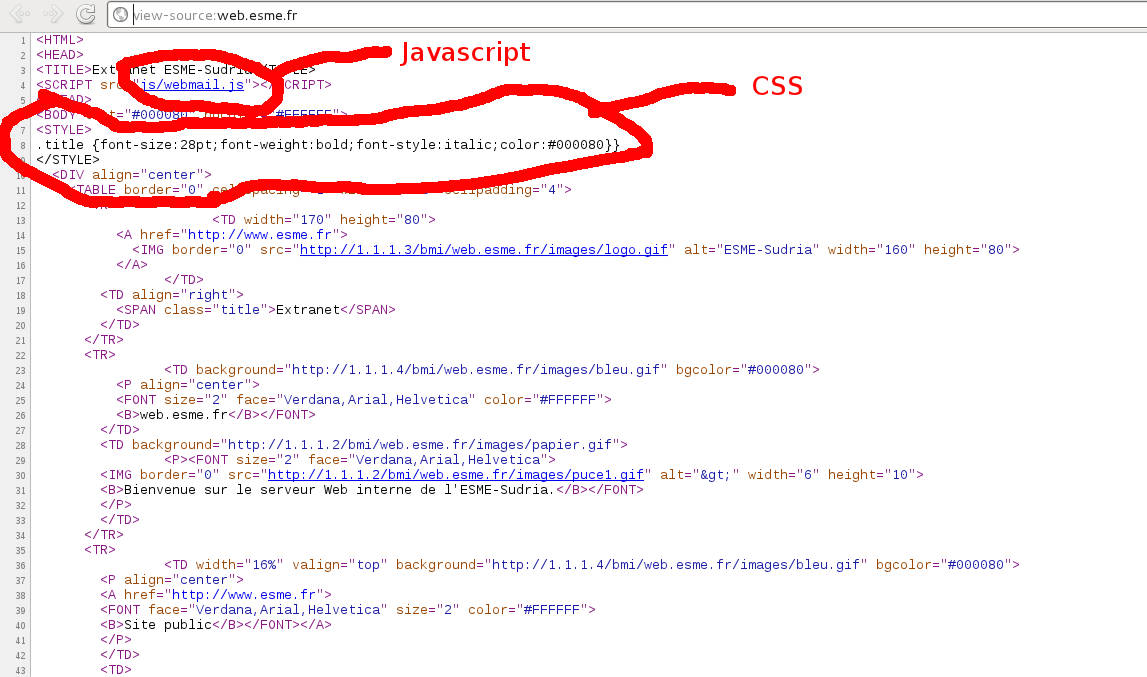
\includegraphics[scale=0.3]{img/html-code-sample.png}
      \caption{Extrait de code HTML contenant du Javascript et du CSS}
      \label{middleware}
    \end{center}
  \end{figure}
}


\ifslide {
  \begin{frame}{HTML, CSS et JavaScript}
    \begin{center}
      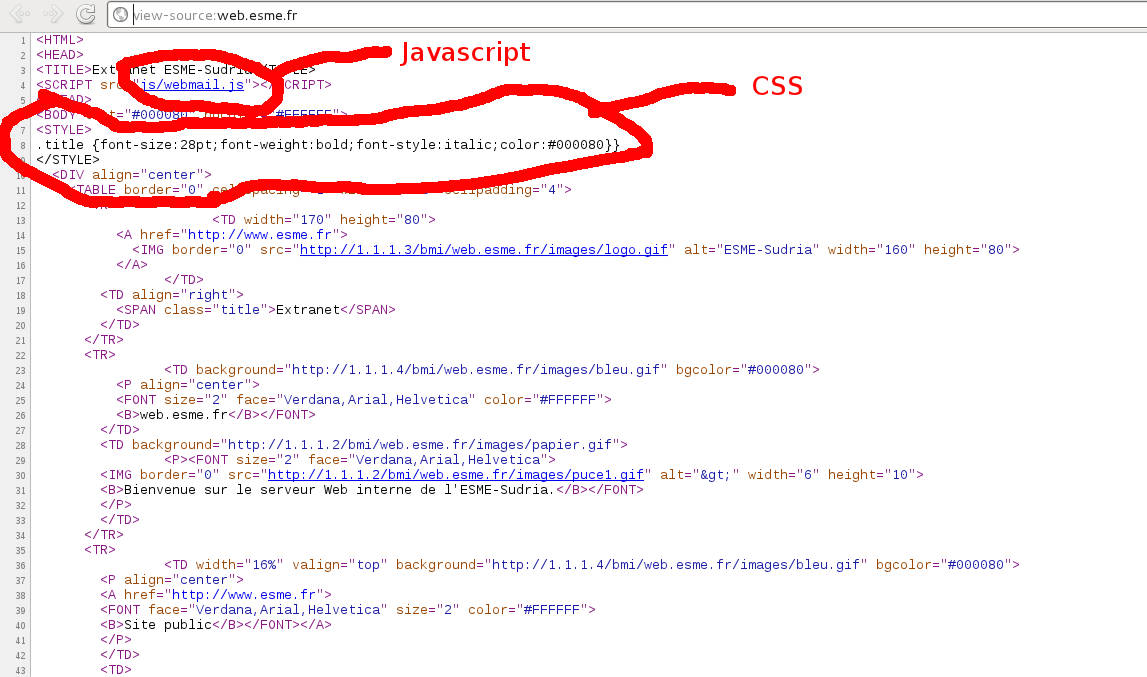
\includegraphics[scale=0.3]{img/html-code-sample.png}
    \end{center}
  \end{frame}
}

\ifbook{
  \paragraph{} En effet, au sein d'une page HTML, on mélange avec allégresse texte avec sa
  présentation qu'il s'agisse de le mettre en gras ou en italique, ou bien de le positionner au sein de la
  page. Et cet état de fait a rendu rapidement très difficile de faire évoluer, du point fonctionnel, les sites -
  puisque les graphistes ou ergonomes ne pouvaient pas travailler de manière indépendante des
  programmeurs, mais aussi de faire évoluer leurs chartes graphiques, puisque leur simple mise à
  jour nécessitait de modifier l'intégralité des pages...

  \paragraph{} C'est ainsi qu'est apparu le CSS, \textit{Cascading Style Sheet}, ou plus
  simplement, les feuilles de styles, dont l'objectif était non seulement de permettre de modifier
  la présentation d'une page HTML existante, mais aussi de séparer la partie présentation d'un site,
  de ses données.

  \paragraph{} En parallèle à l'utilisation du CSS, un autre langage a été introduit, sous forme de
  scripts, placés dans la page, mais dont l'exécution est déclenchée par le navigateur et qui donc
  fonctionne non plus sur le serveur, mais sur le poste client.

  \paragraph{} Introduit tout d'abord de manière propriétaire, ce petit langage permit de rendre les
  sites "web" tellement plus dynamiques et \textbf{conviviaux}, en améliorant grandement
  l'interaction de l'utilisateur avec ces derniers, qu'il fut rapidement adopté, et même normalisé
  sous le nom, rarement utilisé, de ECMAScript.
}

\ifbook {
  \mysubsubsection{Conteneur d'exécution d'application}
  \paragraph{} Comme nous l'avons brièvement résumé, les technologies du "web" se sont construites
  sur une forte volonté d'offrir un système ouvert, standard et interopérable. À l'aide des
  abstractions choisies, et du modèle relativement simple, une page HTML, aussi complexe soit-elle,
  peut être rendue - à peu près, de manière similaire, quelque soit le système d'exploitation
  utilisé.

  \paragraph{} Mais, du coté serveur, les technologies étaient toujours très \textbf{adhérentes} à ce
  dernier. Que vous exécutiez sur Apache HTTP, à l'aide du mod CGI, des scripts Shell sous Unix, ou
  que vous écriviez des pages ASP sur un serveur Microsoft, le code réalisé restait indéniablement
  spécifique à son cadre d'exécution.

  \paragraph{} Progressivement, un certain nombres de cadre d'exécution (et de développements)
  d'application "web" virent le jour, tel que PHP et Java. Ces deux derniers, pour continuer avec
  eux, forment des langages de programmation à part entière, mais le modèle qu'ils proposent apporte
  surtout une réelle interopérabilité coté serveur.

  \paragraph{} En effet, avec ce genre de technologie, il devint possible d'exécuter son programme
  sur n'importe quel type de serveur avec un comportement (presque) identique. On put donc enfin
  aisément migrer de systèmes d'exploitation, dans le cas où celui-ci ne se comporte pas de manière
  suffisante pour l'application, ou recruter un développeur sans que celui-ci n'ai besoin d'autres
  compétences que la seule maîtrise de la technologie.

  \paragraph{} En outre, ces technologies promeuvent, pour la plupart, un certain \textbf{modèle de
  programmation}, et l'écosystème qui les entoure apporte son lot de composants prêts à utiliser
  et destinés à faciliter grandement le développement d'applications "web" robustes et capables de
  monter en charge.

  \begin{figure}[h]
    \begin{center}
      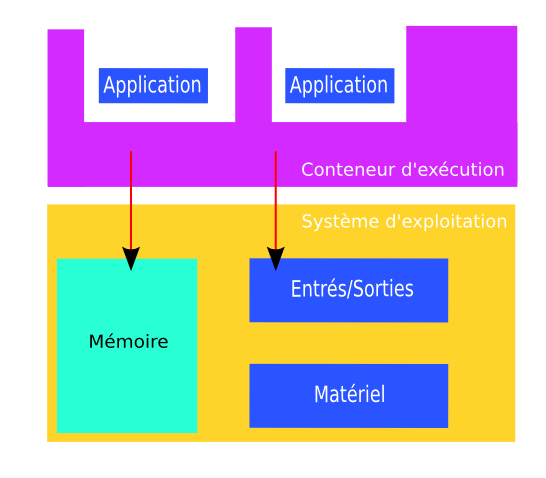
\includegraphics[scale=0.3]{img/execution-container.png}
      \caption{Rôle d'un conteneur d'exécution}
      \label{execution-container}
    \end{center}
  \end{figure}
}


\ifslide {
  \begin{frame}{Conteneur d'exécution}
    \begin{center}
      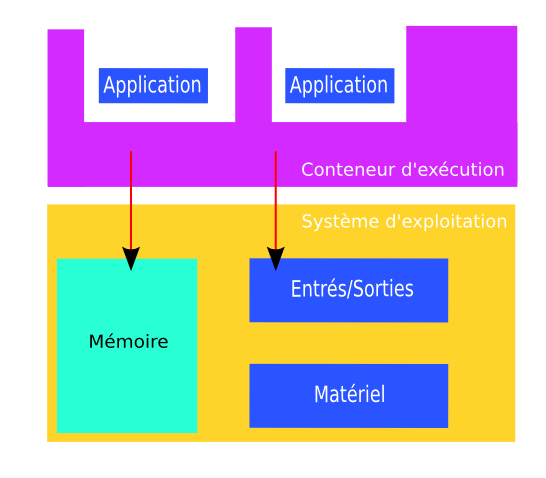
\includegraphics[scale=0.3]{img/execution-container.png}
    \end{center}
  \end{frame}
}

\newpage
\mysubsection{Qu'est ce que le middleware ?}

\ifbook {
  \paragraph{} Après ce vaste état des lieux, nous allons enfin pouvoir rentrer dans le thème de ce
  cours: le \textit{Middleware}. En premier lieu, essayons de trouver une définition un plus parlante
  de ce terme, qui n'a pas réellement de traduction française.

  \paragraph{} Si l'on traduit très littéralement ce terme, on obtient quelque chose de l'ordre du
  "matériel du milieu". Bon, c'est peu parlant, mais clairement le suffixe "\textit{-ware}" fait echo
  aux termes \textit{"software"} - le matériel logiciel, et \textit{"hardware"}, le matériel
  physique, ce qui signifie que, en fait, le mot clé ici, est le "milieu".

  \paragraph{} Mais de quoi exactement sommes-nous au milieu ici ? Revoyons simplement notre dessin
  d'architecture à n-tiers:

  \begin{figure}[h]
    \begin{center}
      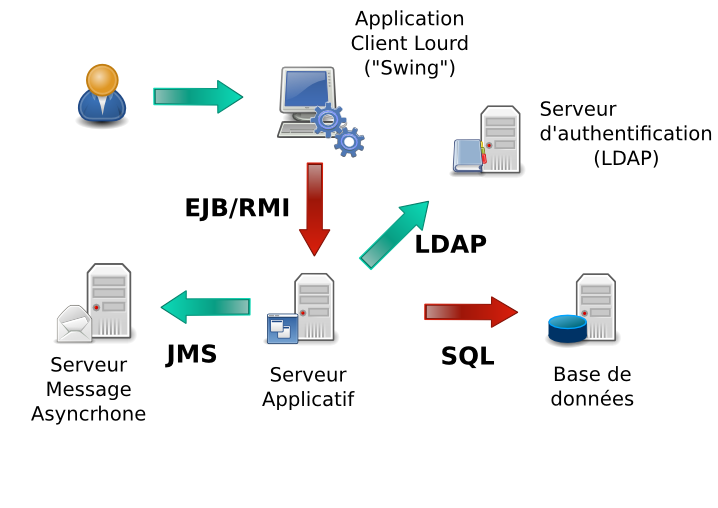
\includegraphics[scale=0.3]{img/n-tiers.png}
      \caption{Où se trouve le middleware sur cette figure ?}
      \label{where-is-middleware}
    \end{center}
  \end{figure}
}

\ifslide{
   \begin{frame}{Qu'est ce que le middleware ?}
     \begin{center}
       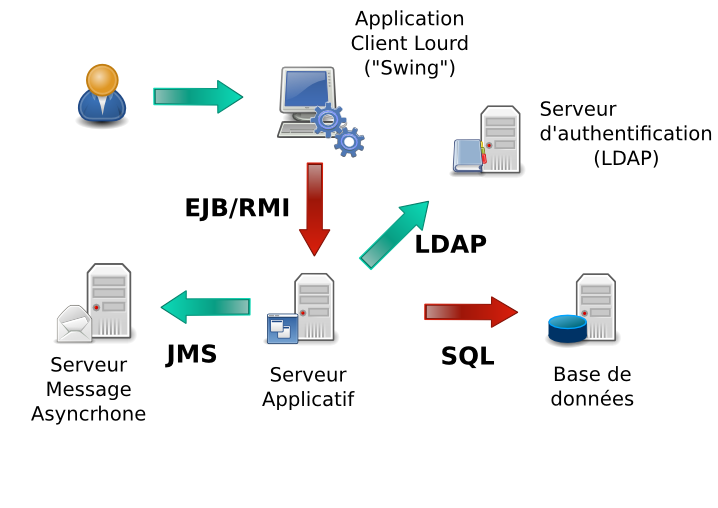
\includegraphics[scale=0.35]{img/n-tiers.png}
     \end{center}
   \end{frame}
}

\ifbook{

  \paragraph{} Le \textit{Middleware} est tout simplement ce qui se retrouve, littéralement, au
  milieu ! Soit entre la base de données et les clients utilisées par les usagers du système. Mais
  au milieu, il y a l'application, non ? Certes oui, mais, celle ci ne s'appuie désormais plus sur les
  seules API fournies par le système d'exploitation, mais sur une kyrielle de services. Ces derniers
  proviennent soit de son environnement d'exécution - tel que une machine virtuelle comme celle de
  Java ou C\#, ou un serveur d'application, ou encore par des composants que l'application elle-même
  embarque.

  \paragraph{} Mais qu'apportent ces services de plus ? Nous allons étudier le "catalogue" en
  détails durant ce cours, mais en quelques mots, ils apportent beaucoup ! Gestion de \textit{pool}
  de connexion, cache locale ou distribué, sécurité, intégration avec un service d'authentification
  distant ou même encore la capacité de mettre en \textit{cluster} l'application pour assurer
  aisément sa montée en charge simplement en ajoutant de nouvelles machines.

  \paragraph{} Pour en revenir à une sorte de définition du \textit{Middleware}, nous retiendrons
  donc que ce dernier est l'ensemble des services utilisées par l'application, aussi bien en son
  sein, que pour communiquer avec des services distants. Bref, en essence, le \textit{Middleware} se
  trouve bel et bien "au milieu", entre l'application et le reste du monde...

  \paragraph{} En essence, le \textit{Middleware}, c'est les briques avec lesquelles on construit
  l'application métier que l'on souhaite réaliser.
  % TODO: dessin fin de déf du middleware: reprendre l'img de plomberie du bootcamp
}
